\section{共享单位读选修复：25 ns 核心时序实际通过}
\label{sec:shared-selector-closure}
在逐行独立读选候选被拥塞否决后，本轮采用另一种只修改装载器的拓扑。
对每个物理行显式定义 \(O_s=W_{s,u}\)，配置读回再从这些行局部旧值中选择
\(O_{s_{cfg}}\)；本行替换直接计算 \(H_s-O_s+W_{new}\)。
因此同一个单位选择器同时服务本行算术和配置读回，行反馈不再穿过全局 slice 选择。
它保留同沿写入、clear 后数值保留、written bitmap、运行锁定和非法地址/值拒绝。
并未减少合法权重精度，也没有新增转换拍或放宽配置路径约束。

最终生产 RTL 的26文件内容摘要为
\par\noindent\code{89b9f8153fea49d82faba8464e45bb83c9}\par\noindent\code{14b11ebf708fb623a9fe3a660b5d26}。
发布代码提交为 \href{https://github.com/defineiocc02/20bit_SAR_ADC_Behaviour_Verification/commit/71e7d5a017246340b9fa1f71cbbe99e20b6503f6}{\code{71e7d5a}}。
该代码的\href{https://github.com/defineiocc02/20bit_SAR_ADC_Behaviour_Verification/actions/runs/36727200500}{CI 36727200500}已完成9/9项工作流，包含22项RTL、3类严格lint及独立40,010个MAC、40,000个ADC2、10,048个除法和8组flags序列检查。测试用合并提交的完整文件树与发布head相同，实际日志和来源见\code{docs/evidence/20260930/ci_shared_71e7d5a/}。
原始综合源包28项中只有\code{rtl/core/weight_store.sv}发生变化，
工具、器件、P5参数、25\,ns XDC 和综合 Tcl 保持相同。
真实实现使用同一个 BUFG 站点、clock uncertainty 和 opt/place/phys\_opt/route 命令；
前代错误的寄存器查询另在同一前代布线DCP上按顺序引脚重算，确保内部hold口径可比。

\begin{table}[H]\centering\small
\begin{tabular}{lrrl}\toprule
同条件测量&前代行缓存&共享读选修复&判断\\\midrule
综合物理LUT&106,205&108,842&增加2,637（2.483\%）\\
综合FF&66,520&66,492&减少28\\
DSP / BRAM / latch&20 / 0 / 0&20 / 0 / 0&保持\\
布线后setup WNS（ns）&$-0.280$&$+0.946$&核心建立时间通过\\
真正寄存器间hold WHS（ns）&$+0.062$&$+0.052$&核心保持时间通过\\
OOC全路径hold WHS（ns）&$-2.361$&$-2.278$&外部接口未闭合\\
路由 / DRC错误&0 / 0&0 / 0&两轮均完成路由\\
\bottomrule\end{tabular}
\caption{Vivado 2018.3、\code{xc7vx690tffg1761-2}、P5、25 ns 的直接对照。setup与hold使用各自最差路径，不将二者合并为一个延迟指标。}
\end{table}

\begin{figure}[H]\centering
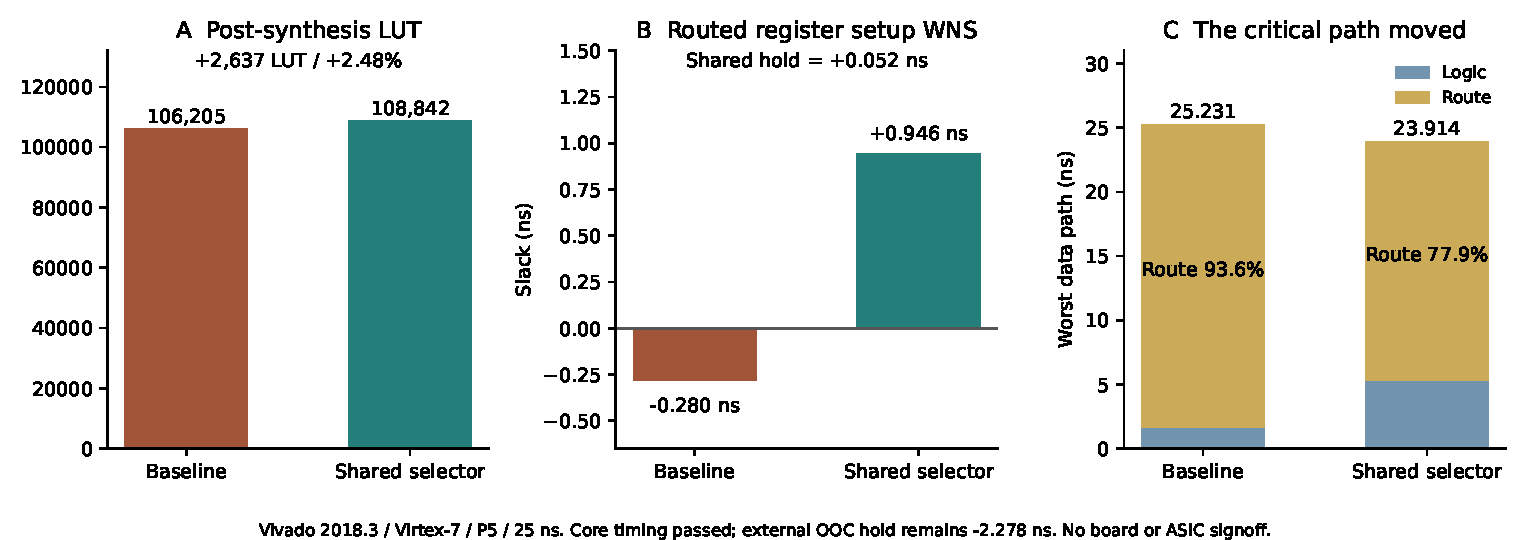
\includegraphics[width=0.98\textwidth]{figures/shared_old_ppa.pdf}
\caption{共享读选的有效综合资源和实际布线时序。生成器逐项核对35+25+40+42个原始证据文件，并绑定两轮DCP、源码差异及XSim来源。末图是两轮各自最差路径，起终点不同，不能当作同一网线延迟削减实验。}
\label{fig:shared-old-ppa}
\end{figure}

新布线报告保留\code{REGREG_TIMING_MET=1}和\code{TIMING_MET=0}，二者并不矛盾。
前者是寄存器clock pin到data pin的setup/hold通过；后者包含零最短输入延迟假设下的外部OOC输入，
仍有65,048个hold失败终点。建立时间失败终点为0，脉宽裕量12.100\,ns，
16类check\_timing问题均为0，路由和DRC错误均为0。
66,508个顺序时钟终点在BUFG插入前后及最终布线后集合完全相同。
这些检查保证所测核心时钟真实布线且顺序边界未被替换，但不是整板IO或模拟比较器接口签核。

25\,ns周期支持记录条件下的40\,MHz核心，固定16拍对应
\(40/16=2.5\,\mathrm{MS/s}\)。本轮没有更高频率的重新实现扫描，
不能用正裕量直接发布更高的保证频率；ASIC的640\,MHz/40\,MS/s仍需目标库与物理实现。
外部hold修复需要发送端最早到达、板级走线、时钟相位和捕获寄存器条件，
不能无依据增加input\_delay、false path或多周期来让总状态变绿。

\subsection{最终源码的逐项RTL图证}
图\ref{fig:shared-ci-arithmetic}--\ref{fig:shared-ci-system}逐项对应最终源码CI的22份原始run log。
生成器核对63个归档payload、88项受测Git输入、每个bench的正常结束和完成标记，
并按原测试台打印的单位呈现计数；没有把check calls、样本、时钟节拍和输入码相加为覆盖率。
历史417f图件仍保留原来源，这里另绘最终71e7版本，不改名冒用旧图。
\begin{figure}[H]\centering
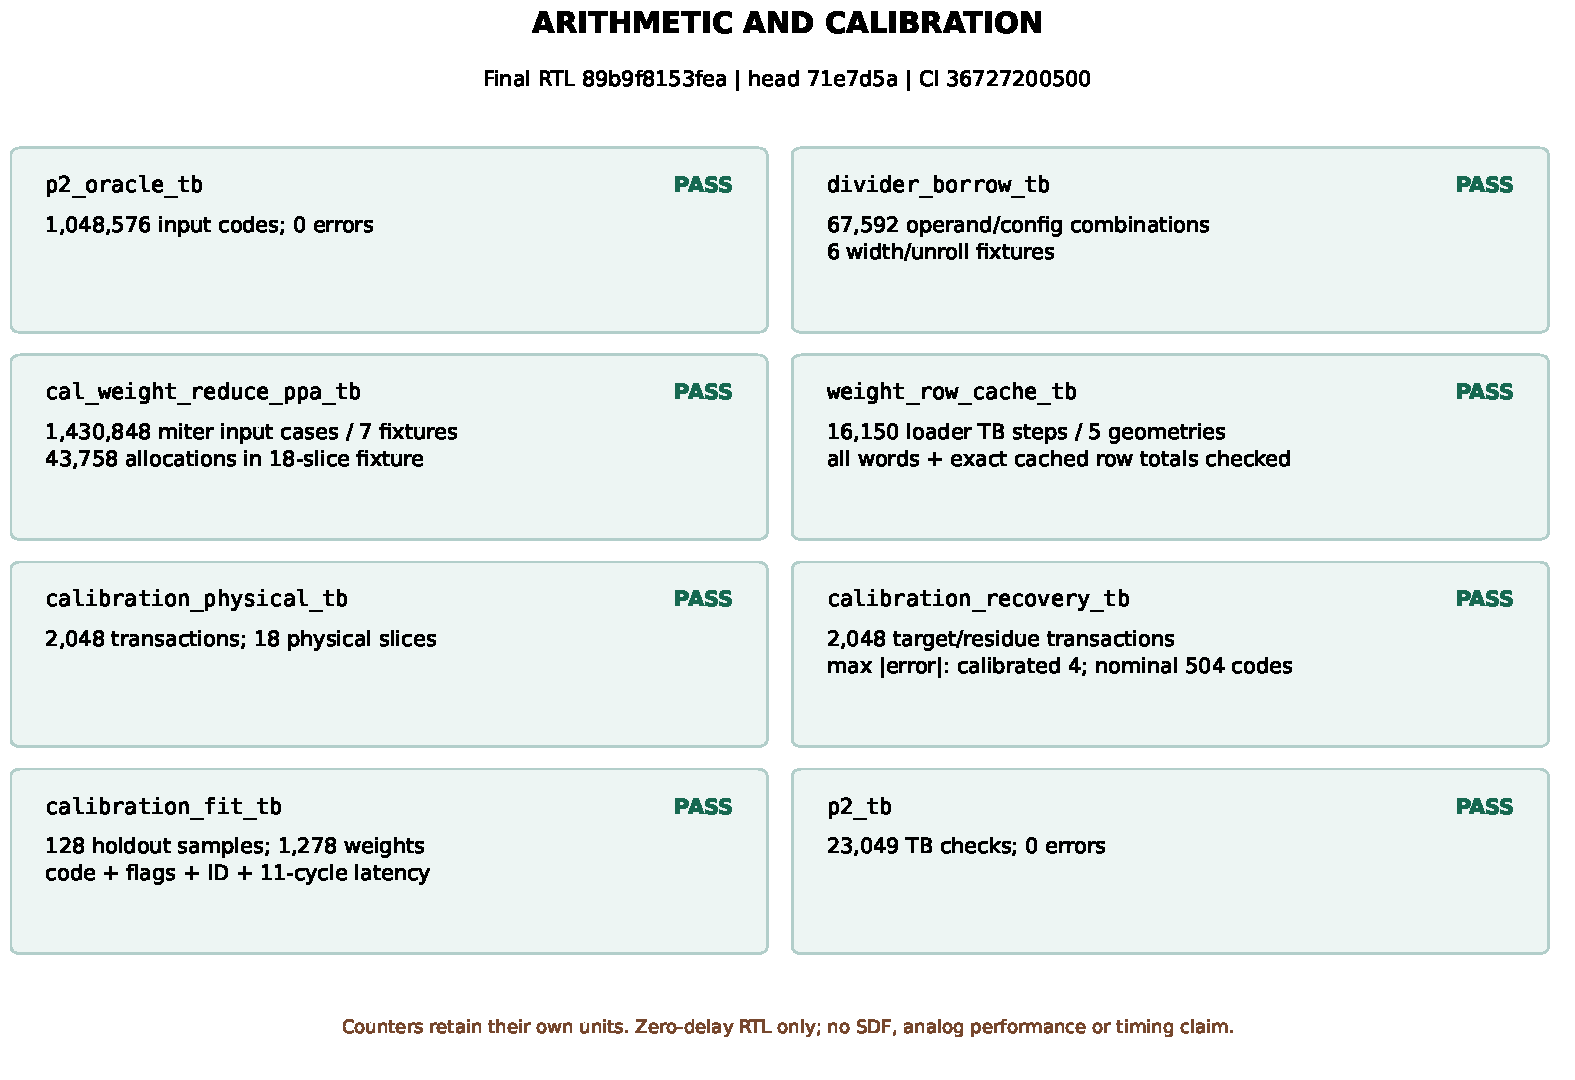
\includegraphics[width=0.98\textwidth]{figures/shared_ci_arithmetic.pdf}
\caption{最终共享读选源码的八项算术/校准RTL证据，包含独立行缓存状态检查、四路归约比较、完整码域简化构造、小位宽除法穷举及标定系数应用。每项仍受本身激励与判据范围限制。}
\label{fig:shared-ci-arithmetic}
\end{figure}
\begin{figure}[H]\centering
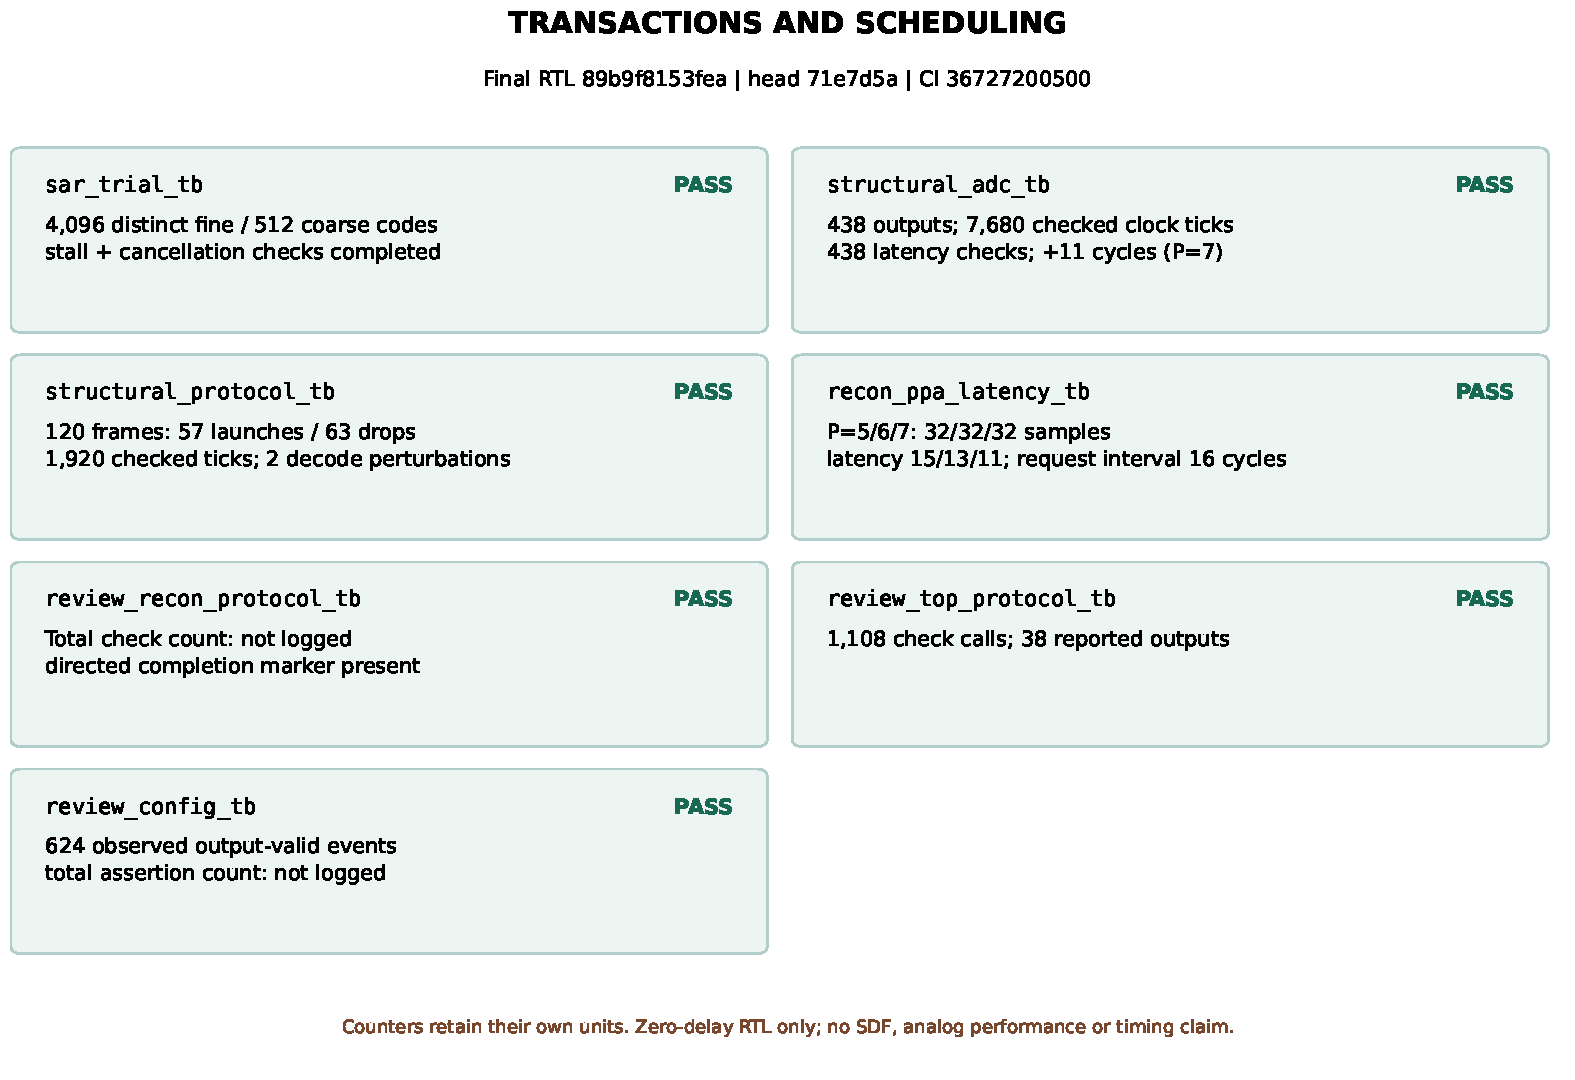
\includegraphics[width=0.98\textwidth]{figures/shared_ci_protocol.pdf}
\caption{最终源码七项事务/调度RTL证据：截止取消、上下文与ID/flags对齐、配置锁定以及三档连续请求。P5/P6/P7各32笔连续请求间隔16拍，输出延迟15/13/11拍；这是功能拍数，不是纳秒时序。}
\label{fig:shared-ci-protocol}
\end{figure}
\begin{figure}[H]\centering
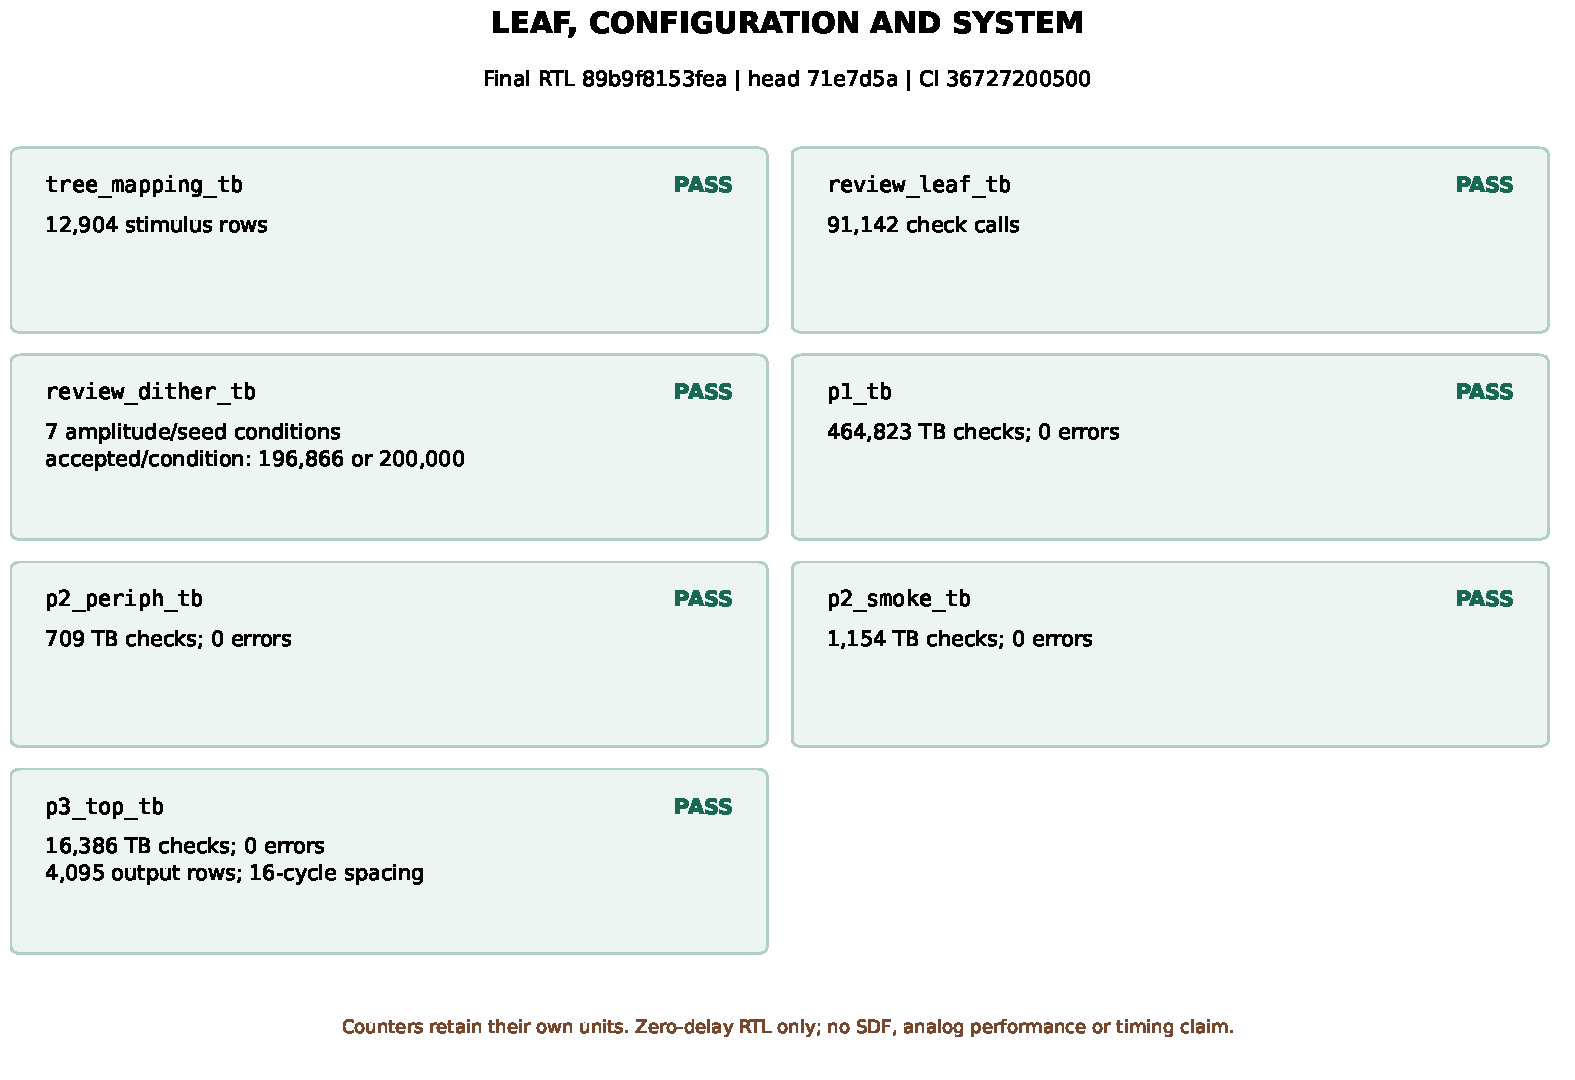
\includegraphics[width=0.98\textwidth]{figures/shared_ci_system.pdf}
\caption{最终源码七项基础/配置/兼容系统RTL证据。P3的4,095输出与16,386次TB检查分别保留单位；tree mapping在此是RTL bench，真正网表结果另列。dither统计来自该测试条件，不能推出模拟动态范围。}
\label{fig:shared-ci-system}
\end{figure}

\subsection{最终源码与完整综合网表的功能链}
\code{shared_old_trial_rtl/}绑定最终26文件源码：官方Verilator 5.020完整22项bench及3类严格lint通过；
P5/P6/P7结构顶层各有438个输出、7,680次协议检查和438笔延迟观测，仍为15/13/11拍。
\code{shared_old_trial_synth/}绑定完全传回并核实的50,563,819字节综合DCP；
\code{shared_old_trial_route_25ns/}从该DCP实施真实BUFG路由；
\code{shared_old_trial_full_mapped/}从同一个综合DCP导出完整功能网表，并在XSim完成仿真。
源码、DCP、生成网表和配置读回测试台的摘要相互核对后才采用这个版本。

\begin{figure}[H]\centering
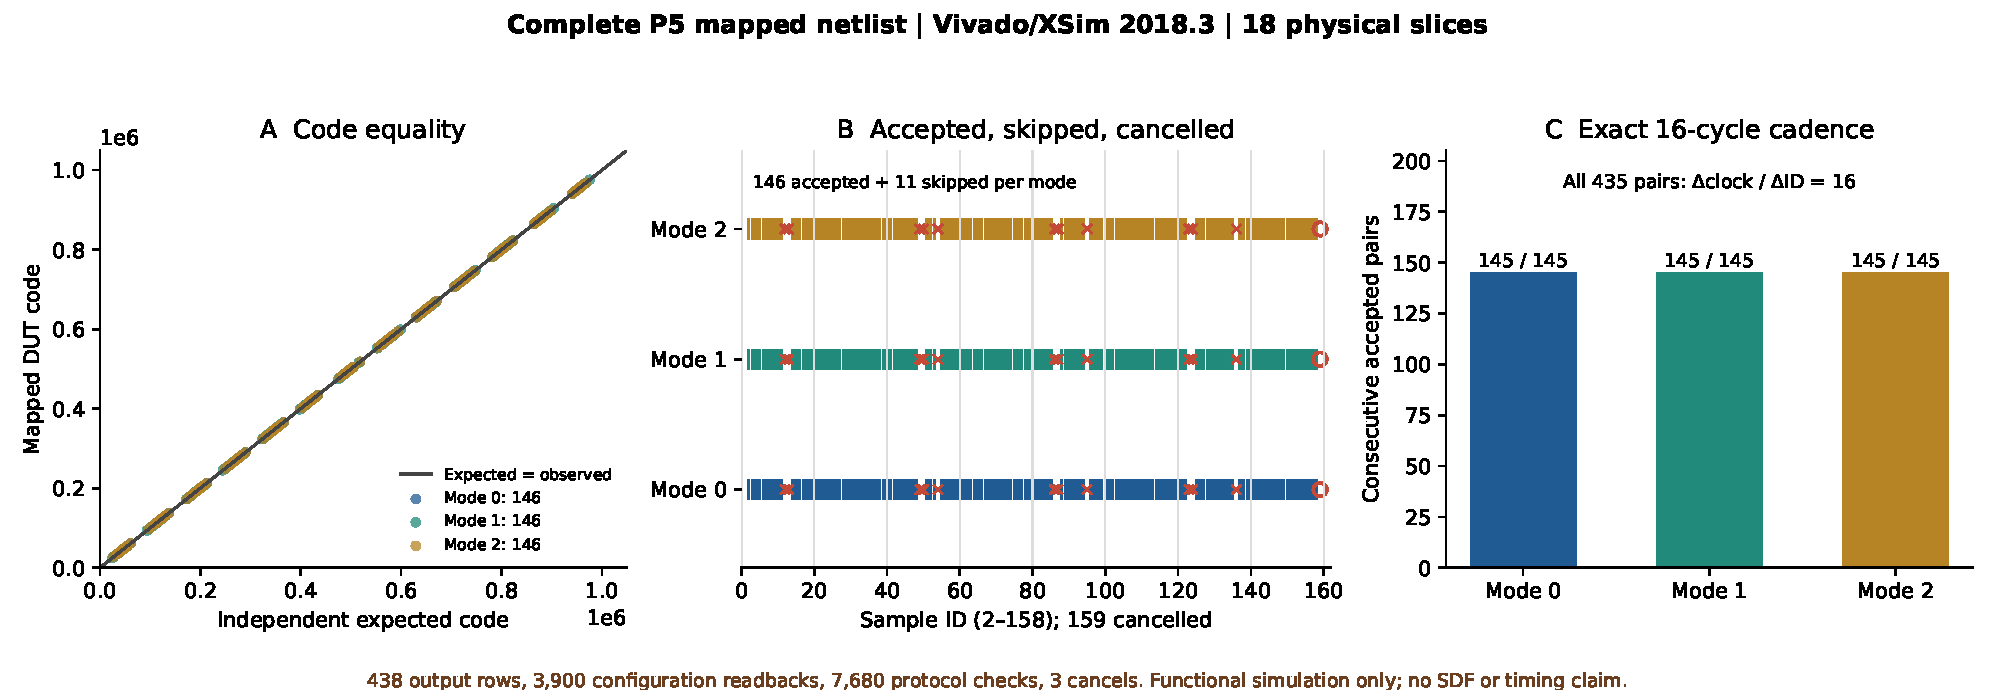
\includegraphics[width=\textwidth]{figures/shared_old_mapped.pdf}
\caption{最终共享读选版本完整P5综合网表的真实公共端口记录：三模式438个code/flags输出、3,900项配置读回、7,680次协议检查及3次取消。全部435对相邻有效输出满足\(\Delta clock=16\Delta ID\)，trace与前代逐字节相同。未作SDF；全部观测flags为0，不能把这张图归为非零异常路径或内部启动延迟覆盖。}
\label{fig:shared-old-mapped}
\end{figure}

完整综合DCP摘要为
\par\noindent\code{63a6faacdc44e54da02514a70ff658ac3}\par\noindent\code{1756853496114513018ac5714cc856e}；
布线DCP摘要为
\par\noindent\code{fba86312b0c96add78ca388b972a52ab7}\par\noindent\code{7c1b781eec34c1b91027b1ea7358072}。
大DCP留在实验目录/远端，Git保留源包、报告、导出身份及运行摘要。
本轮结论是用2.483\%综合LUT代价解决核心setup失败，不能表述为各项PPA同时下降。

\section{进一步PPA优化：先处理已测瓶颈}
\label{sec:further-ppa}
最终最差setup为\code{fine_slices_reg[1][3]}到\code{rails_s_reg[65]}，
数据延迟23.914\,ns，其中逻辑5.291\,ns、布线18.623\,ns（77.875\%），逻辑层数40。
前代最差路径来自配置行更新，93.647\%为布线；局部读选修复以后，
瓶颈已回到样本物理ID、活跃行译码、权重列归约和rail符号处理。
继续只缩短配置加法器不一定提高频率。
\code{flatten_hierarchy rebuilt}会把依赖逻辑重归入层级，
不能把\code{u_context}名下约40,578 LUT解释成上下文寄存器本体需要如此多LUT。
该模块真实状态仅1,422 FF；需根据实际路径和网连接辨认归约逻辑的归属。

\subsection{状态位预算决定面积优化优先级}
权重存储的62,316 FF准确分解为
\begin{equation}
1278\times47+1278\times1+18\times54
=60,066+1,278+972=62,316.
\end{equation}
它占总66,492 FF的93.72\%。只缩小709-bit上下文的两份状态，
或优化少量状态机，无法改变权重表主导的存储成本。
另一方面当前71个单元在所有物理行以并行叶形式供归约使用；
普通双端口存储器不能在同一拍提供这种带宽。
直接把二维packed寄存器改名为RAM而保持全部组合读，不能保证推断出BRAM。
有效方向是先降低每笔校正读取的系数项数，再选择分银行RAM/SRAM和精确的读调度。
若收窄47个合法权重位，必须同步修改量化契约、重新证明数值/拟合误差，
不能依据一次训练样本的最大值就削掉当前公开合法域。

\subsection{利用后级SAR期间预计算，保持样本归属}
\(T,G,R\)在物理开关和配置epoch锁定后即可求出，不依赖后级ADC2最终码\(F\)。
目前前级上下文在相位9捕获，下一笔相位0转交为fine上下文，
后级在相位1--14完成比较，15才启动重构。
因此可评估在后级转换期间分段求局部行和、列和及rail符号，
到phase15只锁存已准备好的\(T,G,R\)与刚完成的\(F\)，继续使用精确MAC和floor除法。
这可以减少启动边沿前的长组合路径；实际收益取决于分段寄存器、布局和扇出。

该候选必须给中间量携带sample ID、epoch、valid和bad状态，
使用已冻结的物理slice ID、主/子开关掩码、dither轨和公共注入，
不能引用正在服务下一笔的实时DEM或RDAC。
clear、disable、迟到比较和cancel要同时清除中间ready，
phase15只允许消费同一ID的完整预计算包；缺包需显式报错并丢弃。
新流水还须检查P5仅一拍余量的busy释放与16拍连续启动，
分别验证数学结果、在途取消、错ID负控及实际setup/hold。
本节是下一步方案，未写入最终RTL，未宣称其已取得频率或面积收益。

\subsection{二维DEM前缀求和：数值等价与存储代价}
本工程主阵列是8\(\times\)8旋转后删去物理单元63，不能直接化为63单元的一维循环。
设行移位\(r_h\)、列移位\(c_h\)，被删物理单元在逻辑展开中的位置为
\begin{equation}
i_*=8((7-r_h)\bmod8)+((7-c_h)\bmod8).
\end{equation}
选择\(n\in[0,63]\)个主单元，相当于在带一个零权重缺位的8\(\times\)8阵列中取前
\(L=n+\mathbf1[n>i_*]\)个逻辑位置。令\(q=\lfloor L/8\rfloor\)、\(k=L\bmod8\)，
加权主和等于从物理行\(r_h\)起的\(q\)个循环整行之和，加上
物理行\((r_h+q)\bmod8\)内从列\(c_h\)起的\(k\)个循环项之和。
对子阵列按\(s_h=\lfloor sid/64\rfloor\bmod8\)作同类查询。

对8项的前缀\(P_j=\sum_{i<j}w_i\)，循环查询为
\begin{equation}
Q(P,a,b)=\begin{cases}P_{a+b}-P_a,&a+b\leq8,\\
P_8-P_a+P_{a+b-8},&a+b>8.\end{cases}
\end{equation}
所以一行的主、子查询至多涉及三个循环段、九个前缀项，
有望替换当前71个on叶的并行归约。但前缀读选、dither保留项、缓存更新和存储银行
都要计算真实端口/面积，不能由读取项数直接推导LUT下降。
兼容模式允许任意开关掩码；此变换只适用于已核对的结构DEM计数，
不能静默套用于任意mask接口。重复/无效物理ID的报警和OR归属也必须保持。

\begin{figure}[H]\centering
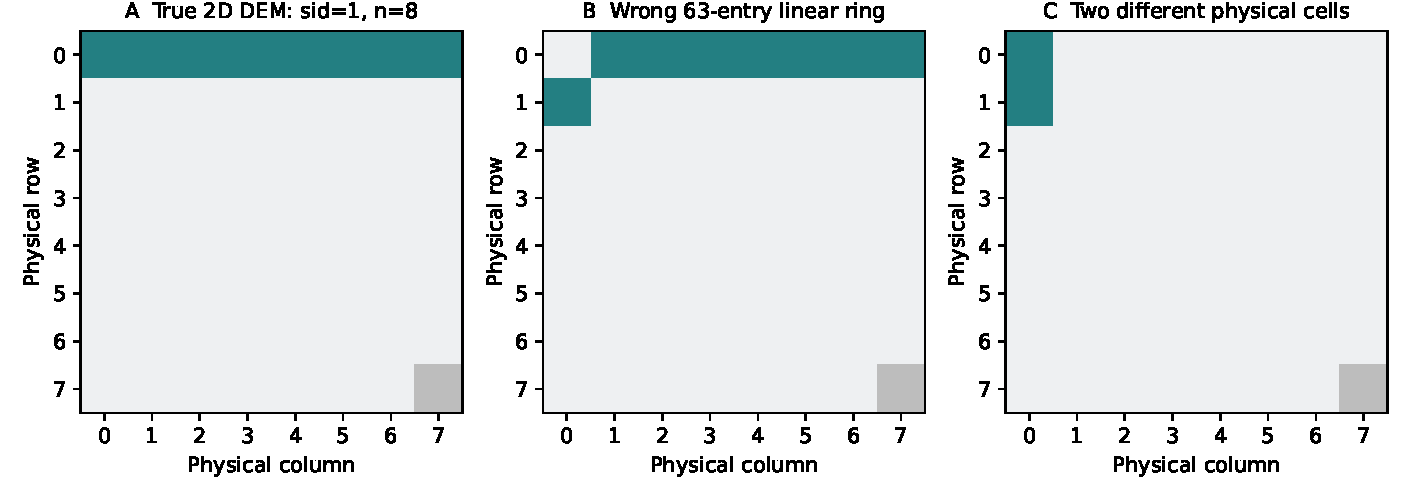
\includegraphics[width=0.97\textwidth]{figures/dem_prefix_math.pdf}
\caption{二维DEM不能直接换为一维环的反例：sid=1、主计数8时，二维方案选择同一行内循环的八项，一维方案则跨到下一行，两项物理单元不同。灰色格为不存在的物理单元63。这是算法结构与错误候选示意，非RTL仿真波形。}
\end{figure}

自写\code{audit_dem_prefix_math.py}以独立Python模型的前向旋转/过滤顺序为oracle，
核对512种DEM状态、64种主计数和8种子计数；91组系数包括71个单项基向量、
全零、全一、全47-bit最大值、递增模式和16组随机值。
主查询2,981,888次、子查询372,736次比较全部相同，一维环负控被拒绝。
基向量覆盖证明固定状态下线性加权选择的项归属；这仍是整数算法见证，不是RTL或综合验收。

保守预算若保留原始权重另加缓存：每slice的8行\(\times\)8个50-bit列前缀为3,200 bit，
8个53-bit整行前缀424 bit，8个50-bit子前缀400 bit，共4,024 bit；
18 slice额外72,432 bit，存储状态从62,316增加到134,748 bit。
因此不能直接追加一套寄存器缓存。
可继续比较用前缀表示\emph{替换}原权重表、配置期串行建表并validate后冻结，
以及分银行SRAM并行读少量前缀项；读回原权重需通过相邻前缀差恢复，
同时重新设计写入完整性、ready、断电恢复、clear语义及dither项访问。
只有上述结构通过完整位精确回归和同约束实现，才可采用。

\subsection{功耗和校准算法的验收边界}
最终布线vectorless报告为0.477 W总功耗、0.152 W动态、0.325 W静态，
报告明确没有Simulation Activity File。权重配置长期保持、校准重构周期活动与
最坏开关模式的翻转分布尚未输入，所以不能据此宣称功耗优势。
下一步应由实际运行模式导出活动数据，分别比较锁定转换、配置装载、DEM/dither和取消，
使用同一活动窗口和板级/工艺条件。

论文的核心数字校准是对已标定物理权重应用精确重构，具体系数求解算法未公开。
本轮保持负数floor、ADC2半值向偶、96-bit域检查和flags语义；
不通过给硬件增加片上LMS/RLS学习器来冒充专利结构复现。
改善标定质量应在片外激励、可辨识性、正值约束、留出集以及PVT漂移上形成独立证据；
改善片上PPA则优先预计算和读取带宽。两类优化分别验收，避免把拟合误差与RTL算术误差混为一类。
